\chapter{Results and Discussion \label{sec:results}}

\section{Testbed Verification \label{sec:testbedResults}}
Before the testbed was used to facilitate comparison between different SDR modules detection performance, its design and components were tested according to the steps in the methodology section. Whilst this was relatively straightforward, it was necessary to ensure the project could meet its aims of a simple, user friendly, potentially scaleable design. 

\subsection{SDR Module Verification \label{sec:sdrVerification}}
The RTL-SDR and LimeSDR Mini were tested to ensure they could be used in the testbed. This comprised of testing both the software driver functionality as mentioned in Section \ref{sec:SDRmodules} and the hardware / communication functionality. 
% RTL SDR TESTING
\par \vspace{0.5cm}
\noindent
\textbf{RTL-SDR}
The RTL-SDR was tested using a combination of librtlsdr command line tools and GQRX, both on the mac and the Rpi5. Starting with the below command to ensure the hardware was detectable:

\begin{verbatim}
    rtl_test -t
\end{verbatim}

\noindent 
In conjunction with the antenna testing below \ref{sec:antennaVerification}, the RTL-SDR waterfall plot was obtained via GQRX, as seen in Figure \ref{fig:rtlSDRwaterfall}.

\begin{figure}[h!]
    \centering
    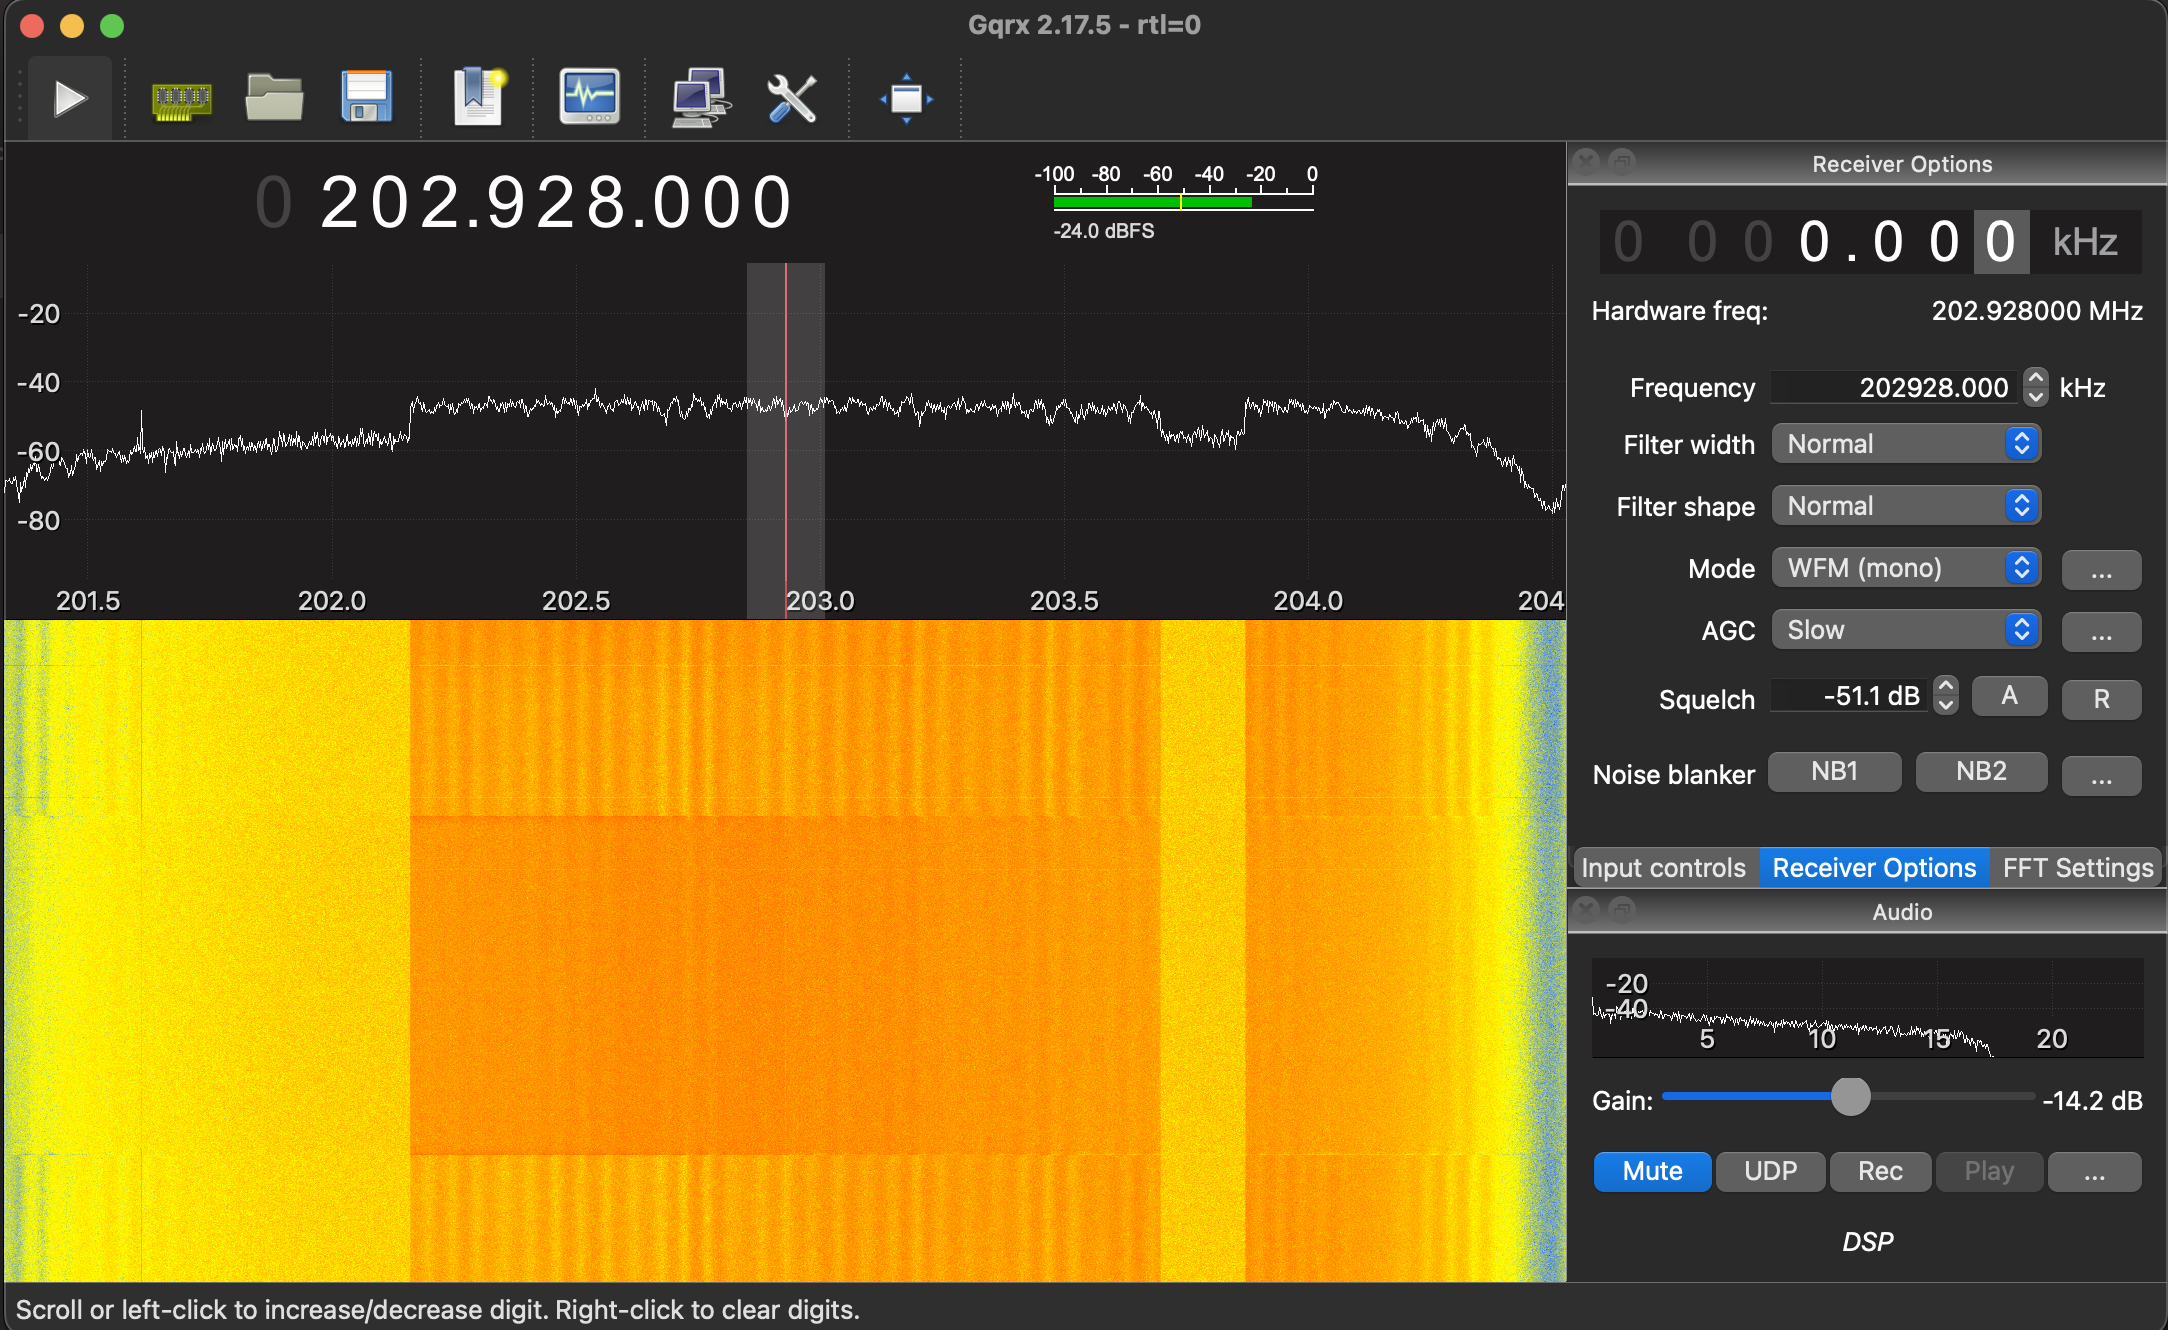
\includegraphics[width=0.6\textwidth]{smaAntennaNF.png}
    \caption{RTL-SDR Waterfall Plot (DAB Multiplex 9A)}
    \label{fig:rtlSDRwaterfall}
\end{figure}

Given that the relevant data processing was to be conducted with a python script, it was also neccessary to test the ability of the RTL-SDR to sample and output data to a .bin file. This was done using the following command:
\begin{verbatim}
    rtl_sdr -s 2048000 -f 202.928e6 -n 2048000 testData.bin 
\end{verbatim}

\noindent
The above test was successful in saving raw IQ data to a .bin file, in the executed directory. Where the saple rate was 2.048 MS/s, the centre frequency was 202.928 MHz (DAB Multiplex 9A) and the number of samples was 2048000 (1 second of data). The \textit{testData.bin} file size for the above example was 4.1MB, highlighting the importance of the storage medium as the sample time is scaled up, as discussed in Section \ref{sec:sbcVerification}.   

\par \vspace{0.5cm}
\noindent
\textbf{LimeSDR}
As with the RTL-SDR, the LimeSDR hardware and software was verified, however it required more effort to test given the relative lack of driver API's. Firstly, the hardware was tested using the Limesuite Hardware API:
\begin{verbatim}
    LimeUtil --find
    LimeQuickTest
\end{verbatim}

\noindent
Which worked to first detect the LimeSDR and then run a series of tests to ensure the hardware was functioning correctly. Specifically the quick test verfied functionality of the clock network, FPGA EEPROM, LMS7002M tuner chip, and the RF loopback. Once the physical hardware was verified it was necessary to ensure that the SoapySDR unifying API was working correctly and could detect the LimeSDR. This was done using the SoapySDRUtil command line tool and output:

\begin{verbatim}
    SoapySDRUtil --find
    ######################################################
    ##     Soapy SDR -- the SDR abstraction library     ##
    ######################################################
    Found device 0
    addr = 1d50:6108
    driver = lime
    label = LimeSDR-USB [USB 3.0] 90706024F3821
    media = USB 3.0
    module = FX3
    name = LimeSDR-USB
    serial = 00090706024F3821
\end{verbatim}

\noindent A python script was then created which utilised the SoapySDR API to sample and save data to a .bin file. The script is viewable in the Appendix \ref{app:limeSDRscript}, this was based on similar code sourced from DeepWave Digital for an Air-T SDR \cite{complexSamplingPython}. It was verified by saving a .bin file and then plotting the PSD of the sample, showing the DAB multiplex centered around 202.928 MHz. Notably, given the LimeSDR has a 12 bit ADC, the output complex IQ data is 32 bits total, with a 16 bit real and 16 bit imaginary component (12 bits zero padded). This resulted in the saved .bin file being 8.2MB for 1 second of data, again showing the high storage requirements for the testbed.

\subsection{RPi5 and NVME Testing \label{sec:sbcVerification}}
In order to compare and quantify the differences in the storage performance between the microSD card and the NVME SSD, a series of tests were conducted, utilising the following linux commands via the terminal of the RPi5.

\begin{verbatim}
    lsblk
    sudo hdparm -t --direct /dev/nvme0n1 
    sudo hdparm -t --direct /dev/mmcblk0
\end{verbatim}
PUT IN RESULTS!!!
\noindent Resulting in the following output seen below in Table \ref{tab:diskperf}.

\begin{table}[h!]
    \centering
    \caption{Disk Read Performance: NVMe vs MicroSD Card \label{tab:diskperf}}
    \begin{tabular}{|l|l|}
    \hline
    \textbf{Device} & \textbf{Read Performance} \\ \hline
    \texttt{NVMe SSD (\texttt{/dev/nvme0n1})} & \texttt{751.22 MB/sec} \\ \hline
    \texttt{MicroSD Card (\texttt{/dev/mmcblk0})} & \texttt{84.83 MB/sec} \\ \hline
    \end{tabular}
\end{table}

The results in Table \ref{tab:diskperf} clearly show the obtained significant performance increase when using the NVME SSD compared to the microSD card. Given the large amount of data that generated and processed during the SDR sampling. 

\subsection{Antenna Testing \label{sec:antennaVerification}}

% IMAGE OF THE NOISE FLOOR COMPARISON

Before calculations or detection was performed, the signal strength of the received signal was measured. This was done by first using the RTL-SDR and the monopole SMA antenna and compared to the Yagi-Uda antenna. The received signal strength, representing the illuminator DAB signal, was measured approximately 6km away from the transmitter tower. \todo{image of maps reference} The results of the signal strength measurements are shown in Table \ref{tab:signalstrength}.

\begin{table}[h!]
    \centering
    \caption{Noise Floor and SNR Comparison with -14.2 dB Gain (RTL-SDR)}
    \label{tab:signalstrength}
    \begin{tabular}{|c|c|c|c|}
        \hline
        \textbf{Antenna Type} & \textbf{Noise Floor (dB)} & \textbf{Signal Strength (dB)} & \textbf{SNR (dB)} \\ \hline
        SMA Monopole & -60 & -40.9 & 19.1 \\ \hline
        Yagi-Uda     & -60 & -17   & 43   \\ \hline
    \end{tabular}
    \vspace{0.5cm}
\end{table}

The above table reflects the high gain of the Yagi-Uda antenna, which is a directional antenna, compared to the monopole SMA antenna. Overall, this testing was valuable to benchmark a noise floor and appreciate the neccessity for a high gain antenna, especially in the context of the low power target signal.

\section{GPIO and Software Excecutable Testing \label{sec:gpioTesting}}

\section{Dection Edge Processing Comparison} \label{sec:edgeProcessing}


\section{RTL-SDR vs LimeSDR Detection Comparison \label{sec:SDRcomparison}}

\section{Overall Design Cost}

\section{Comparison to Existing Work}
% DISCUSS INTEGRATION INTO FLIGHT RADAR 24, etc
